\documentclass{article}

\usepackage[utf8]{inputenc}

\usepackage{nicefrac}
\usepackage{amssymb, amsmath, amsfonts}
\usepackage{amsthm}
\usepackage{tikz}
\usetikzlibrary{matrix,shapes,arrows, calc, intersections}
\usepackage{pgfplots}
\usepgfplotslibrary{groupplots}
\usepackage[a4paper, margin=1in]{geometry}

\newtheorem{proposition}{Proposition}
\newtheorem{theorem}{Theorem}
\newtheorem{definition}{Definition}
\newtheorem{lemma}{Lemma}
\newtheorem{conjecture}{Conjecture}
\newtheorem{corollary}{Corollary}
\newtheorem{remark}{Remark}
\newtheorem{assumption}{Assumption}

\newlength\figureheight
\newlength\figurewidth
\setlength\figureheight{12cm}
\setlength\figurewidth{14cm}

\newcommand{\tikzdir}[1]{tikz/#1.tikz}
\newcommand{\inputtikz}[1]{\input{\tikzdir{#1}}}

\DeclareMathOperator*{\argmin}{arg\; min}     % argmin
\DeclareMathOperator*{\argmax}{arg\; max}     % argmax
\DeclareMathOperator*{\tr}{tr}     % trace
\DeclareMathOperator{\Cov}{Cov}
\DeclareMathOperator{\logdet}{log\;det}

\title{EE8087 Living with Mathematics\\Tutorial 2: Trigonometry II}
\date{}
\begin{document} \maketitle
\begin{enumerate}
\item   A land surveyor wants to determine the height of a building $HG$. She first stands on an adjacent building at point $A$, and measures the angle $\angle GAI$ to be $60^\circ$. She then climbs to a higher position $B$, which is 10 floors above $A$ and the angle $\angle GBI$ is $30^\circ$. She also measures the $\angle HBI$ to be $40^\circ$. Suppose each floor of the building where the land surveyor is on has a height of $3m$. Derive the height of building $HG$.
  \begin{figure}[h]
    \centering
    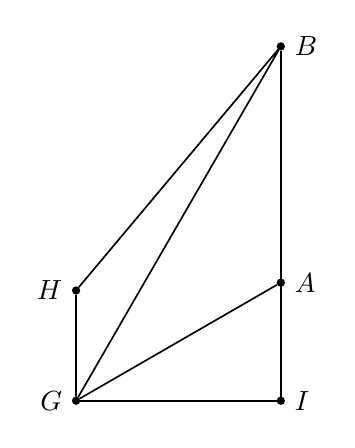
\begin{tikzpicture}[scale=0.1]
      \tikzset{mark coordinate/.style={inner sep=0pt,
          outer sep=0pt,
          minimum size=3pt,
          fill=#1,
          circle}
      }
      \node [mark coordinate=black,label=0:$A$] (A) at (0,15) {}; 
      \node [mark coordinate=black,label=0:$B$] (B) at (0,45) {}; 
      \node [mark coordinate=black,label=0:$I$] (I) at (0,0) {}; 
      \node [mark coordinate=black,label=180:$G$] (G) at (-26,0) {}; 
      \node [mark coordinate=black,label=180:$H$] (H) at (-26,14) {}; 
      \draw [semithick] (B)|-(G);
      \draw [semithick] (H)--(G);
      \draw [semithick] (H)--(B)--(G)--(A);
    \end{tikzpicture}
  \end{figure}
  
\emph{Soln:} Assume that $GI = x$ and $AI= y$. Then we have
\begin{align*}
 \tan 60^\circ = x/y,\, \tan 30^\circ = x/(y+30). 
\end{align*}
Therefore, we have $y = 15$ and $x = 15\sqrt{3}$. Therefore, we can get
\begin{align*}
  HG = BI - GI\cot 40^\circ  = 45 - 15\sqrt{3}\times \cot 40^\circ = 14.04.
\end{align*}

  \newpage

\item A land surveyor wants to measure the width of a river. She finds two points $F$ and $G$ on the opposite banks of the river.  She first stands at position $A$ and measures the angle $\angle GAN$ to be $30^\circ$ and $\angle FAN$ to be $45^\circ$. She then moves to point $B$, which is $100$m to the north of $A$ and $50$m to the east of $A$, and measures the $\angle FBM$ to be $33^\circ$. Derive the width of the river $FG$.
  \begin{figure}[h]
    \centering
    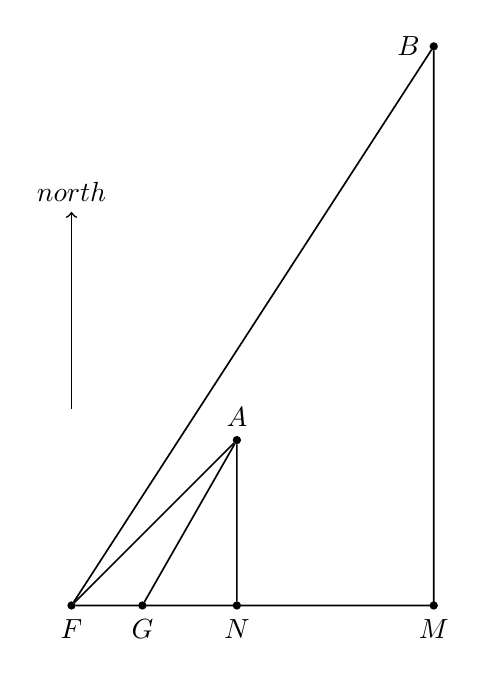
\begin{tikzpicture}[scale=0.05]
      \tikzset{mark coordinate/.style={inner sep=0pt,
          outer sep=0pt,
          minimum size=3pt,
          fill=#1,
          circle}
      }
      \node [mark coordinate=black,label=270:$F$] (F) at (0,0) {}; 
      \node [mark coordinate=black,label=270:$G$] (G) at (18,0) {}; 
      \node [mark coordinate=black,label=270:$N$] (N) at (42,0) {}; 
      \node [mark coordinate=black,label=270:$M$] (M) at (92,0) {}; 
      \node [mark coordinate=black,label=90:$A$] (A) at (42,42) {}; 
      \node [mark coordinate=black,label=180:$B$] (B) at (92,142) {}; 
      \draw [semithick] (F)--(B)|-(F);
      \draw [semithick] (F)--(A)--(N);
      \draw [semithick] (A)--(G);

      \draw [semithick,->] (0,50)--(0,100) node [anchor=270] {$north$};
    \end{tikzpicture}
  \end{figure}
 
\emph{Soln:} Assume that $FN = x$ and $AN= y$. Then we have
\begin{align*}
 \tan 45^\circ = x/y,\, \tan 33^\circ = (x+50)/(y+100). 
\end{align*}
From the first equation, we have $y = x$. From the second equation, we can get
\begin{align*}
  x = \frac{100\tan 33^\circ-50}{1-\tan 33^\circ} = 42.62 = y.
\end{align*}

As a result, $FG = FN-GN = FN- AN\tan 30 = 18.01.$

\newpage
\item An engineer wants to measure the length of a bridge $HK$ that goes across a river. He is standing on a building that is on the bank of the river. Suppose he is at point $A$ and the bottom of building is point $O$. He measures the $\angle KAO = 60^\circ$ and $\angle KAH = 45^\circ$. Then he goes up 10 floors to point $B$, which is $30$m above $A$. He measures the $\angle KBO = 30^\circ$. Derive the length of the bridge $HK$.

   \begin{figure}[h]
    \centering
    \begin{tikzpicture}
      \tikzset{mark coordinate/.style={inner sep=0pt,
          outer sep=0pt,
          minimum size=3pt,
          fill=#1,
          circle}
      }
      \node [mark coordinate=black,label=90:$H$] (H) at (0,3) {}; 
      \node [mark coordinate=black,label=270:$K$] (A) at (0,0) {}; 
      \node [mark coordinate=black,label=270:$building$] (B) at (2.5,0) {}; 
      \draw [semithick] (-4,0)--(4,0);
      \draw [semithick] (-4,3)--(4,3);
      \draw [dashed] (H)--(A);
      \node [anchor=west] at (-4,1.5) {$river$};
    \end{tikzpicture}
  \end{figure}

\emph{Soln:} On the plane of $KBO$, assume that $KO = x$ and $KA = y$. 
   \begin{figure}[h]
    \centering
    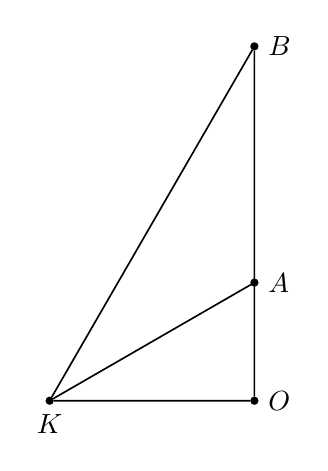
\begin{tikzpicture}[scale=0.1]
      \tikzset{mark coordinate/.style={inner sep=0pt,
          outer sep=0pt,
          minimum size=3pt,
          fill=#1,
          circle}
      }
      \node [mark coordinate=black,label=270:$K$] (K) at (-26,0) {}; 
      \node [mark coordinate=black,label=0:$O$] (O) at (0,0) {}; 
      \node [mark coordinate=black,label=0:$A$] (A) at (0,15) {}; 
      \node [mark coordinate=black,label=0:$B$] (B) at (0,45) {}; 
      \draw [semithick] (K)--(O)--(B)--(K)--(A);
    \end{tikzpicture}
  \end{figure}
Then we have
\begin{align*}
  \tan 60^\circ = x/y,\tan 30^\circ = x/(y+30).
\end{align*}
As a result, $y = 15$ and $x = 15\sqrt{3}$. Hence, $KA = 15/\sin 30^\circ = 30$.

Now since $\angle HKA=90^\circ$ and $\angle KAH = 45^\circ$, we know that $KH = KA = 30m$.
\newpage

 
\item Suppose we have the following sinusoidal single $v_1$ and $v_2$:
\begin{align*}
  v_1 = 3\sin(t),\,v_2 = 4\cos(t+45^\circ).
\end{align*}
Let $v_3 = v_1 + v_2$. Find the maximum value of $v_3$ and the corresponding $t$.

\emph{Soln:} Suppose that $v_3 = A \cos(t + \phi)$, then we have
\begin{align*}
  v_3 = A\cos \phi \cos t - A \sin \phi \sin t = 3\sin t+ 2\sqrt{2}\cos t - 2\sqrt{2} \sin t = 2\sqrt{2}\cos t + (3-2\sqrt{2})\sin t.
\end{align*}
Therefore, we have
\begin{align*}
  A\cos \phi = 2\sqrt{2},\,A\sin \phi = 3-2\sqrt{2}.
\end{align*}
As a result
\begin{align*}
  A = \sqrt{8+(3-\sqrt{8})^2}=2.83,\,\phi = \tan^{-1}\frac{3-\sqrt{8}}{sqrt{8}} = 3.47^\circ.
\end{align*}
As a result, when $t = -3.47+2k\pi$, $v_3$ achieves maximum of $2.83$.
 
\end{enumerate}

\end{document}
%%% Local Variables:
%%% TeX-command-default: "Latexmk"
%%% End:
